%*******************************************
% Lab 08: ALU
%*******************************************
\chapter{Arithmetic Logic Unit (ALU)}\label{alu}

\section{Purpose}

In this lab you will build an \acf{ALU}. An \ac{ALU} is an important digital logic device used to perform all sorts of arithmetic and logic functions in a circuit. The commercial 74181 \ac{ALU} has two four-bit data inputs along with a one-bit mode (M) and a four-bit select input. Depending on those settings, the device will complete one of the functions listed in Table \ref{tab0301}.

\begin{table}[H]
	\sffamily
	\newcommand{\head}[1]{\textcolor{white}{\textbf{#1}}}		
	\begin{center}
		\rowcolors{2}{gray!10}{white} % Color every other line a light gray
		\begin{tabular}{ccc} 
			\rowcolor{black!75}
			\head{Select} & \head{Logic (M=1)} &\head{Arithmetic (M=0)} \\
			0000 & A' & A \\
			0001 & (A + B)' & A + B \\
			0010 & A'B & A + B' \\
			0011 & Logical 0 & minus 1 (2's Comp) \\
			0100 & (AB)' & A + AB' \\
			0101 & B' & (A + B) plus AB' \\
			0110 & A XOR B & A minus B minus 1 \\
			0111 & AB' & AB' minus 1 \\
			1000 & A' + B & A plus AB \\
			1001 & (A XOR B)' & A plus B \\
			1010 & B & (A + B') plus AB \\
			1011 & AB & AB minus 1 \\
			1100 & Logical 1 & A plus A \\
			1101 & A + B' & (A + B) plus A \\
			1110 & A + B & (A + B') plus A \\
			1111 & A & A minus 1
		\end{tabular}
	\end{center}
	\caption{Function Table for 74181 ALU}
	\label{tab0301}
\end{table}

Notes: in the ``Arithmetic'' column, the + sign indicates logic \textit{OR} while the words \textit{plus} and \textit{minus} indicate arithmetic add and subtract operations. The value of \textit{A plus A} is the same as shifting the bits left to the next most significant position.

The \ac{ALU} built in this lab is not as complex as an 74181 \ac{IC}, however it demonstrates the basic functions of an \ac{ALU}.

\section{Procedure}

Load the \ac{ALU} starter circuit in \textit{Logisim-evolution}. 

\subsection{main}

The \lstinline[columns=fixed]|main| circuit does nothing more than provide a human-friendly interface for the rest of the \ac{ALU}. That interface include two eight-bit inputs (labeled \textit{A} and \textit{B}), a three-bit select, a one-bit mode, a carry-in and carry-out bit (so the \ac{ALU} could be chained to another), a \textit{compare} output (TRUE if the two inputs are equal), and a eight-bit output (labeled \textit{ALU\_Out}). In operation, numbers are entered at \textit{A} and \textit{B}, the mode and select are set, and then the result is read on \textit{ALU\_Out}.

\begin{figure}[H]
	\centering
	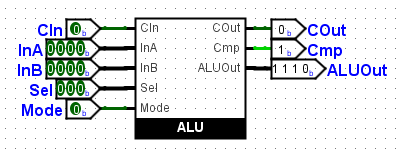
\includegraphics[width=\maxwidth{.95\linewidth}]{gfx/alu-01}
	\caption{ALU main}
	\label{fig:alu-01}
\end{figure}

\subsection{ALU}

The \lstinline[columns=fixed]|ALU| subcircuit is designed to contain the logic that routes \textit{A}, \textit{B}, and \textit{Sel} to two other subcircuits, \lstinline[columns=fixed]|arith\_main| or \lstinline[columns=fixed]|logic\_main|. It then uses a multiplexer to route the output of one of those subcircuits to an output port depending on the setting of the \textit{Mode} bit. Note that the inputs are sent to both subcircuits but only the output specified by the \textit{Mode} is returned to the user. This type of logic is also used in Labs \ref{arith} and \ref{logic}.

The Arithmetic and Logic subcircuits that were built in Labs \ref{arith} and \ref{logic} will be reused for this lab. This is the way that circuit designers can reuse their work to build more complex circuits without having to reinvent the proverbial wheel for every project. To reload those old labs, click \textsc{Project -> Load Library -> Logisim-evolution Library}\footnote{In order to load labs for reuse it is important to store the project files in the same folder.}. Find Lab \ref{arith}, Arithmetic, and click \textit{Open}. That lab is now available as a library in the library list on the left side of the \LE workspace. Follow the same procedure to also load Lab \ref{logic}, Logic, as a library. 

Open the Arithmetic library and drop the \lstinline[columns=fixed]|arithmetic| subcircuit in the \lstinline[columns=fixed]|ALU| subcircuit. This process is exactly like dropping a device from the Wiring library and should not be difficult to figure out. In the same way, drop the \lstinline[columns=fixed]|logic| subcircuit from the Logic library onto the \lstinline[columns=fixed]|ALU| subcircuit.

At this point, the ALU subcircuit should resemble Figure \ref{fig:alu-02}.

\begin{figure}[H]
	\centering
	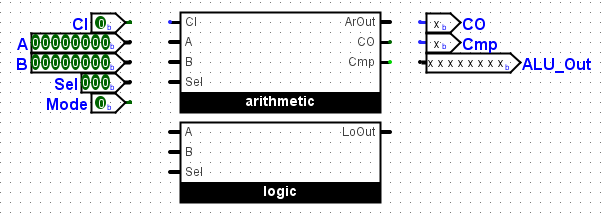
\includegraphics[width=\maxwidth{.95\linewidth}]{gfx/alu-02}
	\caption{ALU Subcircuit}
	\label{fig:alu-02}
\end{figure}

\subsection{Challenge}

Continue to wire the \lstinline[columns=fixed]|ALU| subcircuit. Note: the inputs and outputs that were provided will need to be repositioned in order to complete this build.

\begin{itemize}
	\item Wire the \textit{CI} input to the \textit{CI} port on the \textit{arithmetic} device
	\item Wire inputs A and B to ports \textit{A} and \textit{B} on both devices.
	\item Wire the \textit{Sel} input to the \textit{Sel} ports on both devices.
	\item The \textit{arithmetic} \textit{CO} and \textit{Cmp} ports should be wired to the \textit{CO} and \textit{Cmp} outputs
	\item Add an 8-bit, 2-input multiplexer. The inputs should be wired to the output ports on both devices. The multiplexer select bit should be wired to the \textit{Mode} input. Finally, the multiplexer output should be wired to the \textit{ALU\_Out} output.
\end{itemize}


\subsection{Testing the Circuit}

The \ac{ALU} can be tested from the \lstinline[columns=fixed]|main| circuit. Several values can be entered on \textit{A} and \textit{B} and then various arithmetic and logic operations selected. The outputs for each check should be accurate. A test vector file has been provided for this lab so all of the ALU's functions can be exercised.

\section{Deliverable}

To receive a grade for this lab, complete the Challenge. Be sure the standard identifying information is at the top left of the \textit{main} circuit, similar to this: 

\bigskip
% The minipage environment keeps the three lines together - no page break.
\begin{minipage}{\linewidth}
	\begin{verbatim}
	George Self
	Lab 08: ALU
	February 18, 2018
	\end{verbatim}
\end{minipage}
\bigskip

Save the file with this name: \emph{\texttt{Lab08\_ALU}} and submit that file for grading.
